%\appendix
\section{Trigger Efficiency Model}
\label{sec:appendix_trigger}

As described in Section~\ref{sec:trigSel} we rely on a
mixture of single and double lepton triggers.  The trigger
efficiency is very high because for most of the phase space 
we have two leptons each of which can fire a single lepton 
trigger -- and the single lepton triggers are very efficient.

We apply to MC events a simplified model of the trigger efficiency 
as a function of dilepton species ($ee$, $e\mu$, $\mu\mu$), the $p_T$ 
of the individual leptons, and, in the case of muons, the $|\eta|$
of the muons.  We believe that this model is adequate for
the trigger efficiency precision needed for this analysis.

The model assumptions are the following:

\begin{itemize}

\item Muon and electron trigger turn-ons as a function of $p_T$
are infinitely sharp. {\color{red} Can we add references?}

\item All electron triggers with no ID have 100\%
efficiency for electrons passing our analysis cuts. {\color{red}
Can we add a reference?  Pehaps the top documentation?}

\item Electron triggers with (Tight(er))CaloEleId have 100\%
efficiency with respect to our offline selection.  This we 
verified via tag-and-probe on $Z\to ee$.

\item Electron triggers with EleId have somewhat lower
efficiency.  This was also measured by tag-and-probe.

\item The single muon trigger has 50\% efficiency for 
$|\eta|>2.1$~\cite{ref:evans}.

\item If a muon in fails the single muon trigger, it
will also fail the double muon trigger.  This is actually 
a conservative assumption.

\item The double muon trigger has efficiency
equal to the square of the single muon efficiency.  This is
also a conservative assumption.

\item The $e\mu$ triggers have no efficiency if the muon has $|\eta|>2.1$.
Again, this is conservative.
\end{itemize}

The model also uses some luminosity fractions and some trigger 
efficiencies.

\begin{itemize}

\item $\epsilon_{\mu}$=93\%, the single muon trigger efficiency plateau 
for $|\eta|<2.1$~\cite{ref:evans};

\item $\epsilon'_{\mu}$=40\%, the single muon trigger efficiency plateau 
for $|\eta|>2.1$~\cite{ref:evans};

\item $f9$=0.215: fraction of data with the Mu9 trigger unprescaled.  
(run$\le 147116$).

\item $f11$=0.273 fraction of data with the Mu9 trigger prescaled and
the Mu11 trigger unprescaled.
(147196 $\leq$ run $\leq$ 148058).

\item $e10$=0.002: fraction of data with the 10 GeV unprescaled electron triggers.
(run$\le 139980$).

\item $e15$=0.086: fraction of data with the 15 GeV unprescaled electron triggers.
(139980 $<$ run $\leq$ 144114).

\item $e17$=0.127: fraction of data with the 100\% efficient 17 GeV unprescaled electron triggers.
(144114 $<$ run $\leq$ 147116).

\item $e17b$=0.273: fraction of data with 17 GeV unprescaled electron triggers
with efficiency $\epsilon_e^b=90\%$ (as measured by tag-and-probe).
(147116 $<$ run $\leq$ 148058).

\item $emess$=0.512: the remainder of the run with several different electron
triggers, all of $p_T>17$ GeV.  For this period we measure the 
luminosity-weighted
trigger efficiency $\epsilon(p_T)$ via tag and probe to be 99\% 
($17<p_T<22$, 97\% ($22<p_T<27$), 98\% ($27<p_T<32$) and
100\% ($p_T>32$).

\end{itemize}

The full trigger efficiency model is described separately for 
$ee$, $e\mu$, and $\mu\mu$.

\subsection{$ee$ efficiency model}
\label{sec:eemodel}

This is the easiest.  Throughout the 2010 run we have always 
had dielectron triggers with thresholds lower than our (20,10)
analysis thresholds.  Since electron triggers are very close
to 100\% efficient\cite{ref:evans},
the trigger efficiency for $ee$ is 100\%.  We have verified that 
the efficiency of the dielectron trigger is 100\% with respect 
to the single electron trigger using $Z \to ee$ data.

\subsection{$\mu\mu$ efficiency model}
\label{sec:mmmodel} 

We consider different cases.

\subsubsection{Both muons in $|\eta|<2.1$ and with $p_T>15$ GeV}
This is the bulk of the $\mu\mu$.

\begin{center}
$\epsilon = 1 - (1-\epsilon_{\mu})^2$
\end{center}

\subsubsection{Both muons in $|\eta|<2.1$, one muon with $11<p_T<15$ GeV}
In this case there must be a muon with $p_T>20$ GeV.  The single muon
trigger is operative for the full dataset on this muon.  Some loss
of efficiency can be recovered when the 2nd muon fires the trigger.
But this can happen only for a fraction of the run.  The dimuon trigger
cannot fire in our model to recover any of the efficiency lost by 
the single muon trigger on the high $p_T$ muon.

\begin{center}
$\epsilon = \epsilon_{\mu} + (1-\epsilon_{\mu})\epsilon_{\mu}(f9+f11)$
\end{center}

\subsubsection{Both muons in $|\eta|<2.1$, one muon with $10<p_T<11$ GeV}
Same basic idea as above.

\begin{center}
$\epsilon = \epsilon_{\mu} + (1-\epsilon_{\mu})\epsilon_{\mu}f9$
\end{center}

\subsubsection{Both muons with $|\eta|>2.1$}
This is a very small fraction of events.  
%In our model they can only be triggered by the dimuon trigger.

\begin{center}
$\epsilon = \epsilon_{\mu}^2 + \alpha (1-\epsilon_{\mu}) \epsilon'_{\mu}$
\end{center}

\noindent where $\alpha=2$ if both muons are above 15 GeV, $\alpha=(1+f9+f11)$ if
one of the muons is between 11 and 15 GeV, and $\alpha=(1+f9)$ if one of the muon
is below 11 GeV.

\subsubsection{First muon with $p_T>15$ and $|\eta|<2.1$;  second muon 
with $|\eta|>2.1$}
The single muon trigger is always operative.  If it fails the double muon 
trigger also fails.

\begin{center}
$\epsilon = \epsilon_{\mu} + (1-\epsilon_{\mu})\Delta_{\mu}$
\end{center}

\noindent where

\begin{center}
$\Delta_{\mu} = \epsilon'_{\mu}$ ~~~~(2nd muon with $p_T \geq 15$ GeV) \\
$\Delta_{\mu} = (f9+f11)\epsilon'_{\mu}$ ~~~~(2nd muon with $11 \leq p_T < 15$ GeV) \\
$\Delta_{\mu} = f9\epsilon'_{\mu}$ ~~~~(2nd muon with $9 \leq p_T < 11$ GeV) \\
\end{center}


\subsubsection{First muon with $11<p_T<15$ and $|\eta|<2.1$;  second muon 
with $|\eta|>2.1$ and $p_T>20$}
The single muon trigger at low $\eta$ is fully operative only for a fraction of the run,
this efficiency is captured by the first term below.
For the remaining fraction, we rely on the double muon trigger as well as the 
single muon trigger at high $\eta$ (2nd term in the equation).

\begin{center}
$\epsilon = (f9+f11)(\epsilon_{\mu} + (1-\epsilon_{\mu})\epsilon'_{\mu})
 + (1-f9-f11)(\epsilon_{\mu}^2 + (1-\epsilon_{\mu})\epsilon'_{\mu})$ 
\end{center}

\noindent which reduces to 

\begin{center}
$\epsilon = (f9+f11)\epsilon_{\mu} + (1-f9-f11)\epsilon_{\mu}^2
+ (1-\epsilon_{\mu})\epsilon'_{\mu}$
\end{center}

\subsubsection{First muon with $10<p_T<11$ and $|\eta|<2.1$;  second muon 
with $|\eta|>2.1$ and $p_T>20$}
Same basic idea as above.

\begin{center}
% $\epsilon = f9~\epsilon_{\mu} + (1-f9)\epsilon_{\mu}^2$ 
$\epsilon = f9\epsilon_{\mu} + (1-f9)\epsilon_{\mu}^2
+ (1-\epsilon_{\mu})\epsilon'_{\mu}$
\end{center}

\subsection{$e\mu$ efficiency model}
\label{sec:emumodel}

This is the most complicated case.  The idea is that the muon trigger
is used to get the bulk of the efficiency.  Then the single electron 
trigger(s) and the $e\mu$ triggers are used to get back dome of the 
efficiency loss.  The various cases are listed below.

\subsubsection{Muon with $|\eta|<2.1$ and $p_T>15$}
This is the bulk of the acceptance.

\begin{center}
$\epsilon = \epsilon_{\mu} + (1-\epsilon_{\mu})\Delta_1$ 
\end{center}

where $\Delta_1$ is the efficiency from the electron trigger:
\begin{itemize}
\item $p_T(ele)<15 \to \Delta_1=e10$
\item $15<p_T(ele)<17 \to \Delta_1=e10+e15$
\item $p_T(ele)>15 \to \Delta_1=e10+e15+e17+\epsilon_e^b~e17b+\epsilon(p_T)~emess$
\end{itemize}
 

\subsubsection{Muon with $|\eta|<2.1$ and $11<p_T>15$}

This is the similar to the previous case, except that the muon 
trigger is operative only for a subset of the data taking period.

\begin{center}
$\epsilon = (f11+f9)\epsilon_{\mu} + \Delta_2 + \Delta_3$ 
\end{center}

Here $\Delta_2$ is associated with the period where the muon 
trigger was at 15 GeV, in which case we use electron triggers or
$e\mu$ triggers.  Note that the electron in this case must be
above 20 GeV.  This can happen only in the latter part of the run, 
thus we write
\begin{center}
$\Delta_2 = (1-f11-f9)~(\epsilon_{\mu}~+~
(1-\epsilon_{\mu})\epsilon(p_T))$
\end{center}
\noindent where the first term is for the $e\mu$ trigger and the 
second term corresponds to $e\mu$ trigger failures, in which case we have 
to rely on the electron trigger.

Then, $\Delta_3$ is associated with muon trigger failures in early runs, 
{\em i.e.}, run $<148819$.  In this case the electron trigger picks it 
up and the $e\mu$ trigger does not help.  

\begin{center}
$\Delta_3 = (f11+f9)(1-\epsilon_{\mu}) \cdot \epsilon_e$
\end{center}

\noindent where $\epsilon_e$ is the efficiency of the electron
trigger for $p_T>20$.  This is 100\% up to run 147716 (fraction
$(e10_e15+e17)/(f11+f9)$;  then it is somewhat lower up to
run 148058, then it becomes very close to 100\% again.
For this latter part of the run we approximate it as $\epsilon_e^b$.
Thus:

\begin{center}
$\epsilon_e = (e10_e15+e17)/(f11+f9) + 
\epsilon_e^b(f11+f9-e10-e15-e17)/(f11+f9)$
\end{center}

\subsubsection{Muon with $|\eta|<2.1$ and $9<p_T>11$}

Identical to the previous case, but replace $(f11+f9)$ with $f9$ everywhere.

\subsubsection{Muon with $|\eta|>2.1$}

This is a 10\% effect to start with.  
The first term is from the electron efficiency.  The 2nd term is the correction
due to the single muon efficieny. 

\begin{center}
$\epsilon = \Delta_1 + (1-\Delta_1)\Delta_{\mu}$
\end{center}

\subsection{Summary of the trigger efficiency model}
\label{sec:trgeffsum}

We take the trigger efficiency for $ee$ as 100\%.  The trigger efficiency
for the $e\mu$ and $\mu\mu$ final states is summarized in 
Figures~\ref{fig:emuModel} and~\ref{fig:mumuModel}.
We estimate the systematic uncertainties on the trigger modeling 
to be at the few percent level.

\begin{figure}[htb]
\begin{center}
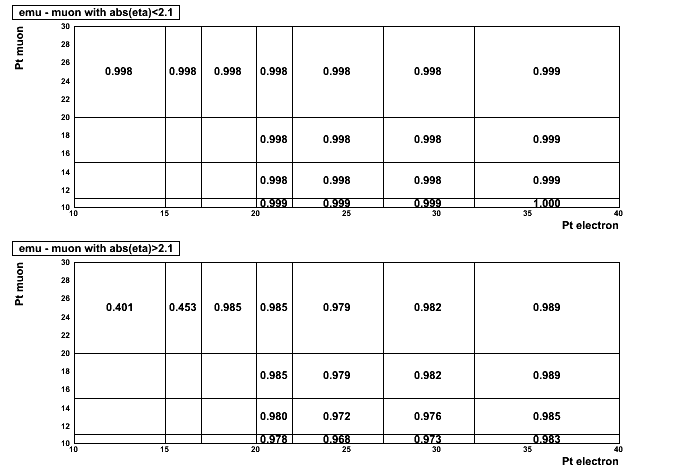
\includegraphics[width=0.99\linewidth]{emuModel.png}
\caption{\label{fig:emuModel}\protect Trigger efficiency for the
$e\mu$ pair as a function of the $p_T$ of the two leptons.
The top table corresponds to $|\eta(\mu)| < 2.1$, the bottom
table to $|\eta(\mu)| > 2.1$.} 
\end{center}
\end{figure}
\clearpage


\begin{figure}[tbh]
\begin{center}
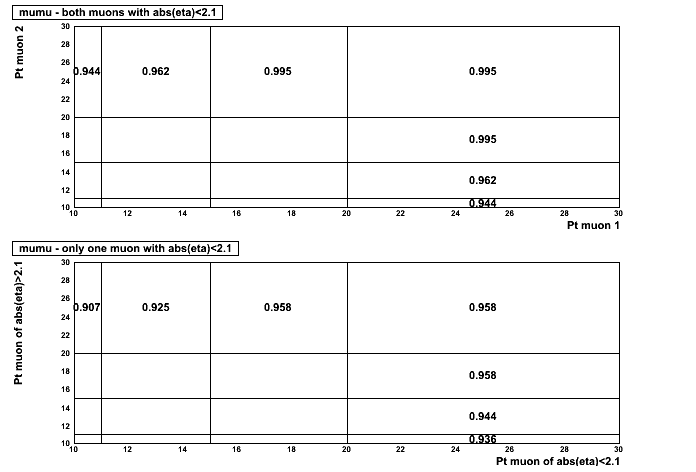
\includegraphics[width=0.99\linewidth]{mumuModel.png}
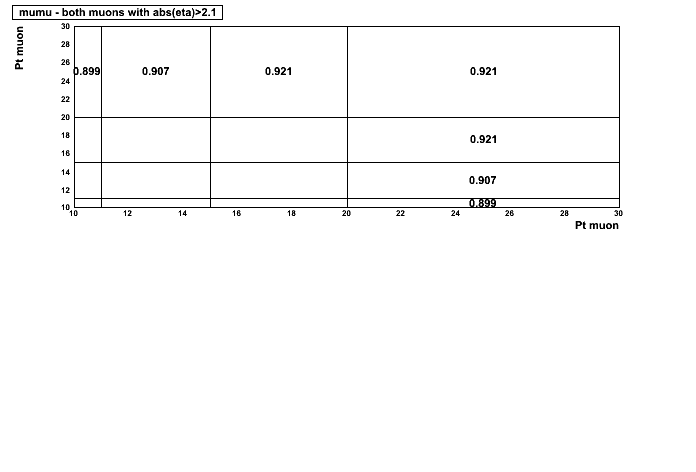
\includegraphics[width=0.99\linewidth]{mumu24Model.png}
\caption{\label{fig:mumuModel}\protect Trigger efficiency for the
$\mu\mu$ pair as a function of the $p_T$ of the two muons.
The top table corresponds to both muons having $|\eta| < 2.1$;
the middle table has one of the muon with $|\eta|<2.1$ and the
other muon with $|\eta|>2.1$; the bottom table has both muons with 
have $|\eta|>2.1$.}
\end{center}
\end{figure}

\clearpage